\documentclass[xcolor=dvipsnames,table]{beamer}

\usepackage{latexsym}
\usepackage[utf8]{inputenc}
\usepackage[brazil]{babel}
\usepackage{amssymb}
\usepackage{amsmath}
\usepackage{stmaryrd}
\usepackage{fancybox}
\usepackage{datetime}
\usepackage[T1]{fontenc}
\usepackage{graphicx}
\usepackage{graphics}
\usepackage{url}
\usepackage{algorithmic}
\usepackage{algorithm}
\usepackage{acronym}
\usepackage{array}

\newtheorem{definicao}{Definio}
\newcommand{\tab}{\hspace*{2em}}

\mode<presentation>
{
  \definecolor{colortexto}{RGB}{0,0,0}
 
  \setbeamertemplate{background canvas}[vertical shading][ bottom=white!10,top=white!10]
  \setbeamercolor{normal text}{fg=colortexto} 

  \usetheme{Warsaw}
}

\title{Apresentação da disciplina} 

\author{
  Esdras Lins Bispo Jr. \\ \url{bispojr@ufg.br}
  } 
 \institute{
  Teoria de Grafos \\Bacharelado em Ciência da Computação}
\date{\textbf{02 de maio de 2015} }

\logo{
\includegraphics[width=1cm]{images/ufgJataiLogo.png}}

\begin{document}

	\begin{frame}
		\titlepage
	\end{frame}

	\AtBeginSection{
		\begin{frame}{Sumário}%[allowframebreaks]{Sumário}
    		\tableofcontents[currentsection]
    		%\tableofcontents[currentsection, hideothersubsections]
		\end{frame}
	}

	\begin{frame}{Plano de Aula}
		\tableofcontents
		%\tableofcontents[hideallsubsections]
	\end{frame}
	
	\section{Sobre a Disciplina}
	\subsection{Professor}
	\begin{frame}{Professor}
		\begin{columns}
			\column{.4\textwidth}  		
		  		\begin{center}
		    		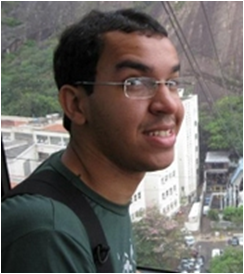
\includegraphics[height=.5\textheight]{images/esdras.png}
		  		\end{center}
			\column{.6 \textwidth}  		
				\begin{block}{Formação}
					\begin{center}
						{\normalsize {\bf Bacharel} em Sistemas de Informação\\
						{\bf Mestre} e {\bf Doutorando} em Representação Conhecimento (IA)}
					\end{center}
				\end{block}		  		
		  		\begin{block}{Quem?}
		  			\begin{center}
						{\bf Esdras Lins Bispo Junior} \\ Recife, Pernambuco.
					\end{center}
				\end{block}
		\end{columns}
	\end{frame}
	
	\begin{frame}{Professor}
		\begin{center}
    		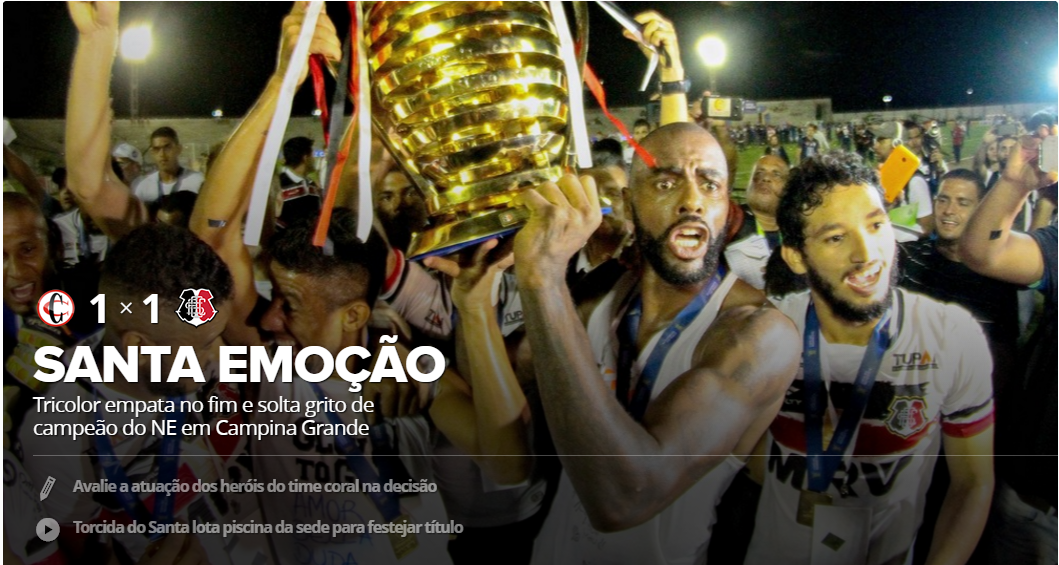
\includegraphics[height=.65\textheight]{images/santa.png}
  		\end{center}
	\end{frame}
	
	\subsection{Informações Importantes}
	\begin{frame}{Informações Importantes}
		\begin{block}{Professor}
			\begin{itemize}
				\item Esdras Lins Bispo Jr.
				\item \url{bispojr@ufg.br}
				\item Sala 18, 1º Andar (Bloco Novo dos Professores)
			\end{itemize}
		\end{block}
	\end{frame}	
	
	\begin{frame}{Informações Importantes}
		\begin{block}{Disciplina}
			\begin{itemize}
				\item Teoria de Grafos
				\item 13h30-15h10 (Segunda, LEC III)\\
					  13h30-15h10 (Terça, LEC III)
				\item Dúvidas: 15h30 - 17h10 (Segunda)\\
					  {\color{red}[é necessário confirmação comigo]}
				\item \url{www.facebook.com/groups/tg.rej.2016.1/}
			\end{itemize}
		\end{block}
	\end{frame}
	
	\begin{frame}{Informações Importantes}
		\begin{block}{Metodologia}
			\begin{itemize}
				\item Aulas expositivas;
				\item Testes;
				\item Prova;
				\item Exercícios.
			\end{itemize}
		\end{block}
	\end{frame}
	
	\begin{frame}{Informações Importantes}
		\begin{block}{Testes}
			\begin{itemize}
				\item Teste 1 $\Rightarrow$ 20\% da pontuação total (16 de maio);
				\item Teste 2 $\Rightarrow$ 20\% da pontuação total (13 de junho);
				\item Teste 3 $\Rightarrow$ 20\% da pontuação total (28 de junho);
				\item Teste 4 $\Rightarrow$  20\% da pontuação total (08 de agosto).
			\end{itemize}
		\end{block}
		\begin{block}{Avaliação}
			\begin{itemize}
				\item Prova $\Rightarrow$  20\% da pontuação total (16 e 30 de agosto).
			\end{itemize}
		\end{block}
		\begin{block}{Exercícios [Bônus]}
			\begin{itemize}
				\item Somatório dos exercícios.
			\end{itemize}
		\end{block}
	\end{frame}
    
    \begin{frame}[shrink]{Informações Importantes}
		\begin{block}{Exercícios-Bônus}
			\begin{itemize}
				\item Semanalmente serão disponibilizados exercícios-bônus (EB) valendo 0,5 ponto na média (segunda-feira, normalmente); \pause
                \item Será dado um prazo para as candidaturas\\
                (normalmente um dia); \pause
                \item Será dada prioridade às candidaturas aos seguintes alunos: \pause
                	\begin{enumerate}
                    	\item Respondeu a nenhum EB; \pause
                        \item Respondeu a um EB; \pause
                        \item Respondeu a dois EBs; \pause
                        \item e assim por diante.
                    \end{enumerate} \pause
                \item Haverá sorteio entre candidatos dentro da mesma prioridade; \pause
            	\item Uma semana após, o candidato apresentará a sua resposta [texto escrito e slides] (normalmente na segunda, 15h30).
			\end{itemize}
		\end{block}
	\end{frame}
	
	\begin{frame}{Informações Importantes}
		\begin{block}{Avaliação}
			O cálculo da média final será dada da seguinte forma:
			\begin{itemize}
				\item MF = MIN(10, PONT)
			\end{itemize}
			em que MIN representa o mínimo entre dois valores e PONT representa a pontuação total obtida em toda a disciplina.
		\end{block} \pause
		\begin{exampleblock}{Previsão de Término das Atividades}
			06 de setembro de 2016
		\end{exampleblock}
	\end{frame}

	\begin{frame}{Informações Importantes}
		\begin{block}{Conteúdo do Curso}
			\begin{enumerate}
				\item Noções Básicas de Grafos;
				\item Circuitos e Caminhos;
				\item Subgrafos;
				\item Grafos Conexos e Componentes;
				\item Cortes e Pontes;
			\end{enumerate}
		\end{block}
	\end{frame}
	
	\begin{frame}{Informações Importantes}
		\begin{block}{Conteúdo do Curso}
			\begin{enumerate}
				\item Árvores;
				\item Isomorfismo;
				\item Coloração;
				\item Planaridade;				
				\item Outros Tópicos.
			\end{enumerate}
		\end{block}
	\end{frame}

%------------------------------------------
	\section{Pensamento}
	\begin{frame}{Pensamento}
  		\begin{center}
    		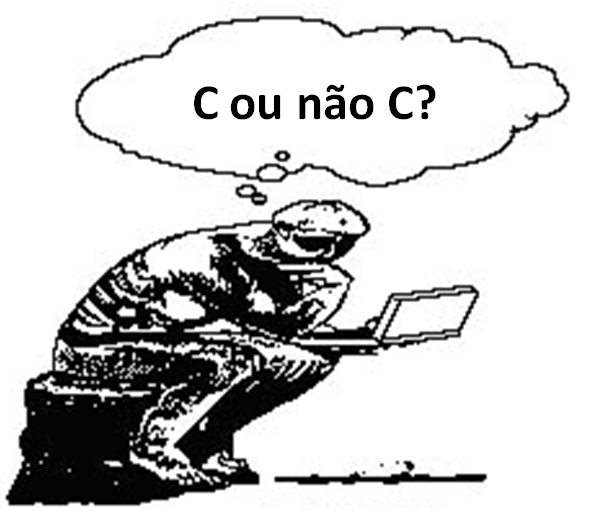
\includegraphics[width=7cm]{images/pensamento.png}
  		\end{center}
	\end{frame}
	
	\begin{frame}{Pensamento}
		\begin{columns}
			\column{.4\textwidth}  		
		  		\begin{center}
		    		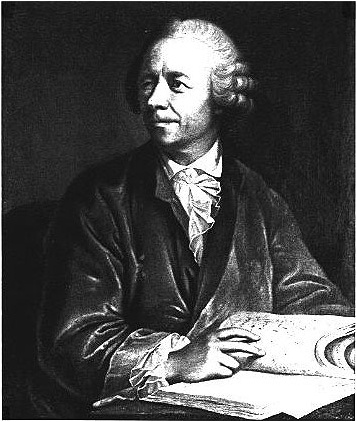
\includegraphics[height=.5\textheight]{images/euler.png}
		  		\end{center}
			\column{.6\textwidth}  		
				\begin{block}{Frase}
					\begin{center}
						{\large Now I will have less distraction.}
					\end{center}
				\end{block}		  		
		  		\begin{block}{Quem?}
		  			\begin{center}
						{\bf Leonhard Euler (1707-83)} \\ Matemático e físico suíço.
					\end{center}
				\end{block}
		\end{columns}
	\end{frame}
%------------------------------------------
	\section{O problema de Euler}
	\begin{frame}[shrink]{O problema de Euler}
		\begin{center}
    		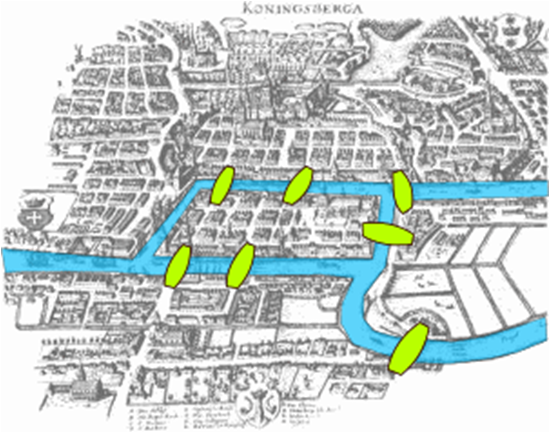
\includegraphics[height=.6\textheight]{images/konigsberg.png}
  		\end{center} \pause
		\begin{alertblock}{Sete pontes de Konigsberg} \pause
			É possível cruzar as setes pontes sem passar \\
			duas vezes por nenhuma delas?
		\end{alertblock}
	\end{frame}
	
	\begin{frame}[shrink]{O problema de Euler}
		\begin{center}
    		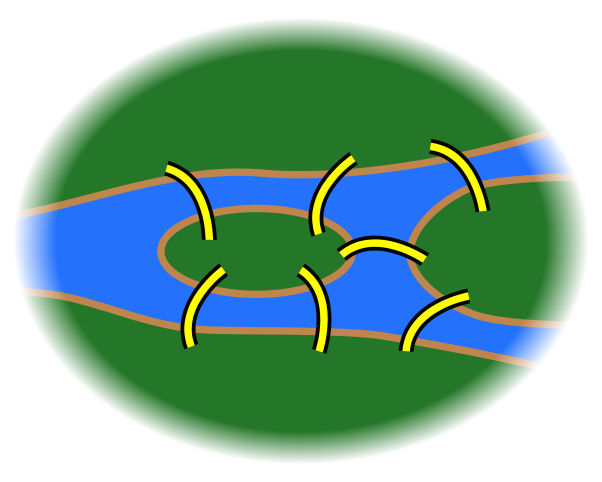
\includegraphics[height=.6\textheight]{images/konigsberg2.png}
  		\end{center} 
		\begin{alertblock}{Sete pontes de Konigsberg} 
			É possível cruzar as setes pontes sem passar \\
			duas vezes por nenhuma delas?
		\end{alertblock}
	\end{frame}
	
	\begin{frame}{O problema de Euler}
		\begin{center}
    		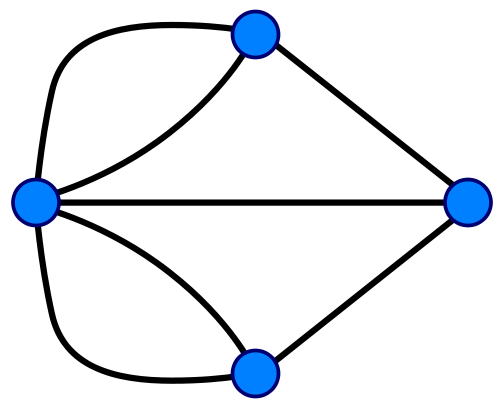
\includegraphics[height=.6\textheight]{images/konigsberg3.png}
  		\end{center} 
		\begin{block}{Sete pontes de Konigsberg} \pause
			Apresentado em 1736.
		\end{block}
	\end{frame}
	
	\section{O problema de Guthrie}
	\begin{frame}[shrink]{O problema de Guthrie}
		\begin{center}
    		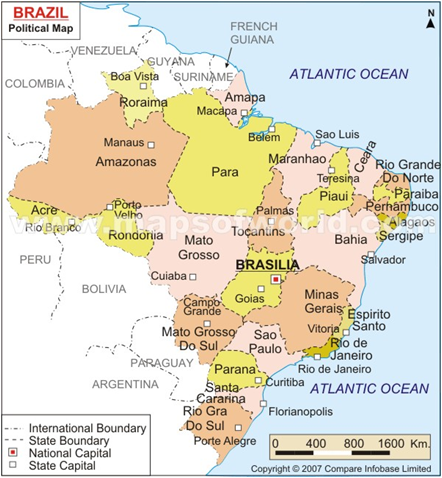
\includegraphics[height=.6\textheight]{images/mapa.png}
  		\end{center} \pause
		\begin{alertblock}{Coloração de Mapas} \pause
			É verdade que quatro cores são suficientes \\
			para se colorar um mapa plano?
		\end{alertblock}
	\end{frame}
	
	\begin{frame}[shrink]{O problema de Guthrie}
		\begin{center}
    		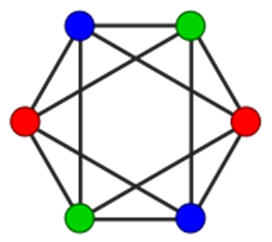
\includegraphics[height=.6\textheight]{images/grafoColorido.png}
  		\end{center}
		\begin{alertblock}{Coloração de Mapas}
			É verdade que quatro cores são suficientes \\
			para se colorar um mapa plano?
		\end{alertblock}
	\end{frame}
	
	\begin{frame}{O problema de Guthrie}
		\begin{center}
    		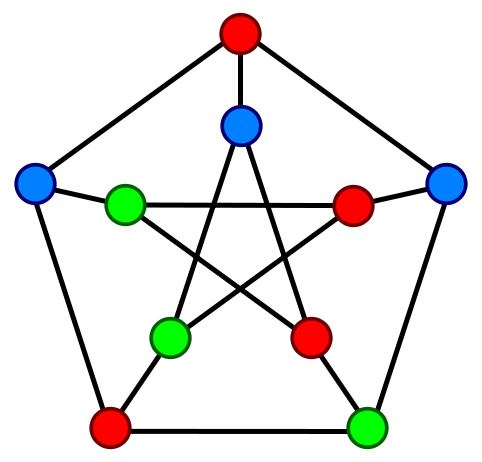
\includegraphics[height=.6\textheight]{images/grafoColorido2.png}
  		\end{center}
		\begin{block}{Coloração de Mapas} \pause
			Apresentado em 1852. Provado em 1976.
		\end{block}
	\end{frame}
	
	\section{O problema do menor caminho}
	\begin{frame}{O problema do menor caminho}
		\begin{center}
    		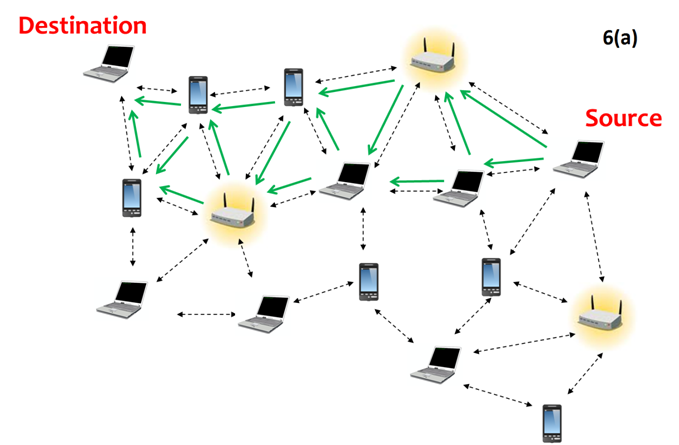
\includegraphics[height=.6\textheight]{images/redes.png}
  		\end{center}
		\begin{alertblock}{Menor Caminho} \pause
			Qual é o roteamento de menor custo entre dois dispositivos?
		\end{alertblock}
	\end{frame}
	
	\begin{frame}{O problema do menor caminho}
		\begin{center}
    		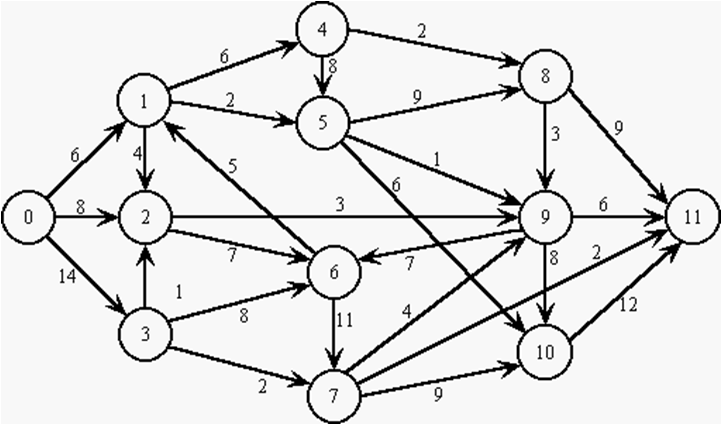
\includegraphics[height=.6\textheight]{images/redesGrafo.png}
  		\end{center}
		\begin{block}{Menor Caminho} \pause
			Algoritmo de Dijkstra (proposto em 1959).
		\end{block}
	\end{frame}
	
	\begin{frame}{O que existe em comum nos três problemas?} \pause
		\begin{block}{Modelo} \pause
			Um modelo é uma {\bf simplificação} da realidade. Um modelo abstrai algumas informações e se concentra em outras informações.
		\end{block} \pause
		\begin{block}{Bom modelo}
			Um bom modelo é aquele que consegue descrever com maior proximidade as características essenciais do problema.
		\end{block}
	\end{frame}
	
	\section{Noções Básicas de Grafos}	
	\begin{frame}{Noções Básicas de Grafos}
		\begin{block}{$V^{(2)}$}
			Para qualquer conjunto $V$, denotaremos por $V^{(2)}$ o conjunto de todos os pares não-ordenados de elementos distintos de $V$.
		\end{block}
	\end{frame}
	
    \begin{frame}{Bônus (0,5 pt)}
		\begin{block}{Desafio}
			\begin{itemize}
				\item Mostre que $\sqrt{2}$ é um irracional; \pause
                \item Candidaturas até amanhã (03 de maio, 13h30); \pause
                \item Apresentação e resposta por escrito $\rightarrow$ \\segunda (10 de maio, 15h30); \pause
                \item 20 minutos de apresentação.
			\end{itemize}
		\end{block} \pause
        \begin{block}{Referência}
			FEOFILOFF, P. {\bf Exercícios de Teoria dos Grafos}, \\
			BCC, IME-USP, 2012. \\ 
			\color{blue}{\url{http://www.ime.usp.br/~pf/grafos-exercicios/}}.
		\end{block}	
	\end{frame}
	
	\begin{frame}
		\titlepage
	\end{frame}
	
\end{document}